%------------------------------------------------------------------------------
% Template file for the submission of papers to IUCr journals in LaTeX2e
% using the iucr document class
% Copyright 1999-2011 International Union of Crystallography
% Version 1.4a (17 April 2011)
%------------------------------------------------------------------------------

\documentclass[pdf]{iucr}           % DO NOT DELETE THIS LINE

     %-------------------------------------------------------------------------
     % Information about the type of paper
     %-------------------------------------------------------------------------
     \paperprodcode{a000000}      % Replace with production code if known
     \paperref{xx9999}            % Replace xx9999 with reference code if known
     \papertype{CP}               % Indicate type of article
                                  %   FA - research papers (full article)
                                  %   SC - short communications
                                  %   LA - lead article
                                  %   FE - feature articles
                                  %   ST - structural communications
                                  %   XC - crystallization communications
                                  % (Following categories rarely in LaTeX)
                                  %   AA - abstracts
                                  %   AD - addenda and errata
                                  %   BC - books received
                                  %   BR - book reviews
                                  %   CA - cif applications
                                  %   CE - current events
                                  %   CI - inorganic compounds
                                  %   CM - metal-organic compounds
                                  %   CN - cryocrystallography papers
                                  %   CO - organic compounds
                                  %   CP - computer programs
                                  %   CR - crystallographers
                                  %   CS - scientific comment
                                  %   ED - editorial
                                  %   EI - inorganic compounds
                                  %   EM - metal-organic compounds
                                  %   EO - organic compounds
                                  %   FI - inorganic compounds
                                  %   FM - metal-organic compounds
                                  %   FO - organic compounds
                                  %   IP - issue preface
                                  %   IU - iucr
                                  %   LE - letters to the editor
                                  %   LN - laboratory notes
                                  %   ME - forthcoming meetings/short courses
                                  %   MR - meeting reports
                                  %   NN - notes and news
                                  %   NP - new commercial products
                                  %   OB - obituaries
                                  %   SR - software reviews
                                  %   TE - teaching and education

     \paperlang{english}          % Can be english, french, german or russian
     %-------------------------------------------------------------------------
     % Information about journal to which submitted
     %-------------------------------------------------------------------------
     \journalcode{J}              % Indicate the journal to which submitted
                                  %   A - Acta Crystallographica Section A
                                  %   B - Acta Crystallographica Section B
                                  %   C - Acta Crystallographica Section C
                                  %   D - Acta Crystallographica Section D
                                  %   E - Acta Crystallographica Section E
                                  %   F - Acta Crystallographica Section F
                                  %   J - Journal of Applied Crystallography
                                  %   S - Journal of Synchrotron Radiation
          %--------------------------------------------------------------------
          % The following entries will be changed as required by editorial staff
          %--------------------------------------------------------------------
     \journalyr{2011}
     \journaliss{1}
     \journalvol{67}
     \journalfirstpage{000}
     \journallastpage{000}
     \journalreceived{0 XXXXXXX 0000}
     \journalaccepted{0 XXXXXXX 0000}
     \journalonline{0 XXXXXXX 0000}

\usepackage{url, hyperref}

\begin{document}                  % DO NOT DELETE THIS LINE

     %-------------------------------------------------------------------------
     % The introductory (header) part of the paper
     %-------------------------------------------------------------------------

     % The title of the paper. Use \shorttitle to indicate an abbreviated title
     % for use in running heads (you will need to uncomment it).

\title{Dataflow: a Web-based Data Reduction Framework for Neutron Scattering}
%\shorttitle{Short Title}

     % Authors' names and addresses. Use \cauthor for the main (contact) author.
     % Use \author for all other authors. Use \aff for authors' affiliations.
     % Use lower-case letters in square brackets to link authors to their
     % affiliations; if there is only one affiliation address, remove the [a].

\cauthor[a]{William}{Ratcliff}{william.ratcliff@nist.gov}{}
\author[a]{Brian}{Maranville}
\author[a]{Paul}{Kienzle}
\author[a,b]{Andrew}{Tracer}
\author[a]{Ophir}{Lifshitz}
\author[a]{Elakian}{Kanakaraj}
\author[a]{Brendan}{Rowan}
\author[a]{Alex}{Yee}
\author[c]{Joseph}{Redmon}

\aff[a]{National Institute of Standards and Technology, Gaithersburg, Maryland  20899 \country{USA}}
\aff[b]{Princeton University, Princeton, NJ  08544 \country{USA}}
\aff[c]{Unknown}

     % Use \shortauthor to indicate an abbreviated author list for use in
     % running heads (you will need to uncomment it).

%\shortauthor{Soape, Author and Doe}

     % Use \vita if required to give biographical details (for authors of
     % invited review papers only). Uncomment it.

%\vita{Author's biography}

     % Keywords (required for Journal of Synchrotron Radiation only)
     % Use the \keyword macro for each word or phrase, e.g. 
     % \keyword{X-ray diffraction}\keyword{muscle}

%\keyword{keyword}

     % PDB and NDB reference codes for structures referenced in the article and
     % deposited with the Protein Data Bank and Nucleic Acids Database (Acta
     % Crystallographica Section D). Repeat for each separate structure e.g
     % \PDBref[dethiobiotin synthetase]{1byi} \NDBref[d(G$_4$CGC$_4$)]{ad0002}

%\PDBref[optional name]{refcode}
%\NDBref[optional name]{refcode}

\maketitle                        % DO NOT DELETE THIS LINE

\begin{synopsis}
Supply a synopsis of the paper for inclusion in the Table of Contents.
\end{synopsis}

\begin{abstract}
Neutron scattering is a technique which necessarily requires centralized facilities, 
with  distributed access (a user facility).  At such a facility, 
outside users collect data on one or more
instruments, which is typically recorded in instrument-specific coordinates.
Each user needs to do two things with this data: convert it into more universal
(physical) coordinates, and correct for any instrumentation-specific artifacts
in the data. This process is termed ``data reduction''.
A common paradigm for data reduction is for the instrument operator to create a
new program and interface for each instrument. The source
data files are reduced at user facility, where there is direct access to both
the programs and the data. The reduced output files are then carried home by the
users.
This project aims to simplify this part of the user experience. A
visual-programming interface is created in the user's browser, allowing
reduction of the source data by remote control. Reduction protocols are built up
using facility-supplied functions (in icon form) wired together to create a data
flow diagram. The user (or instrument operator) can change the reduction
protocol, and repeat the procedure as needed, and the resultant reduced files
can be downloaded by the users at will. Standard reduction protocols are made
available by the facility and instrument operator.
Changes to the protocol (and the addition of new instruments and new protocols)
will not require changes to the user interface, and instrument-specific
functions for reduction will be maintained by the instrument operators, rather
than a full-blown unique reduction program for each instrument or type of
instrument.
\end{abstract}


     %-------------------------------------------------------------------------
     % The main body of the paper
     %-------------------------------------------------------------------------
     % Now enter the text of the document in multiple \section's, \subsection's
     % and \subsubsection's as required.

\section{Introduction}

Every dataset that is produced at a neutron user facility must be reduced to physical coordinates,
with artifacts removed and error bars added, before it can be analyzed or modeled.
As a result, every instrument is typically equipped with a software routine for performing this 
reduction.  In addition, if the reduction programs are to be distributed to the users so that
they might work with the raw data at their home institutions after the experiment is complete,
each program must be compiled for multiple target platforms 
(Microsoft Windows, Mac OS, Unix, Linux, etc.).  
At a large facility this requires the writing and maintenance of dozens of programs, with multiple
target platforms for each program, just to perform reduction.
Updates to software are also on a per-instrument basis, requiring
notification of all the users who might have downloaded or copied the programs, requesting that they 
download a newer version.

For this reason, the Dataflow framework was designed to consist of two parts: 
the user interface which exists solely within the user's web browser, and a centralized server which
is maintained by the facility staff.  Updates to the server are implemented without needing
interaction from the user, and updates to the user interface code (in the browser) require only that 
the user refresh their view of the reduction site.
 

\section{Client}

By presenting the user interface in a web browser, the installation requirement for users is shifted to the
browser providers.  All that is required of the user is that they run a modern browser.
Current browser support is indicated in Table \ref{table_browsers}.
The user interface is built in Javascript, mainly using the WireIt and ExtJS libraries.
Plotting is accomplished through custom-built plugins for the jqPlot library 
(\url{http://www.jqplot.com/}), which is built on another common Javascript library, jQuery.




\section{Server}

The Dataflow system was designed with a backend server written in Python (Django, \url{http://www.djangoproject.com}),
which makes the connection between the client (web browser) and the data reduction modules, which are written 
in Python.  There is no particular requirement that the reduction code be written in Python, just that
the code be callable from Python.  Because of the large available body of numerical libraries 
in Python, it was not necessary to use any other languages in the project.  

\subsection{Instrument-specific modules}

In the client and server, every reduction pipeline is categorized in terms of a single ``instrument''.
For each instrument, all the reduction subroutines and data formats are defined.  Typically this will
consist of one or more ``loaders'' which import raw data from datafiles, and ``filters'' which operate
on the data.  It is necessary that the loaders and filters provide compatible objects within each
instrument's namespace, but it is not required that the filters for one instrument operate on the data
of another instrument.  Thus every reduction problem is able to be addressed individually on the backend
without requiring modification of the data or file types already in use.  

All that is required is that
existing algorithms for data reduction be ported to individual Python modules that act as filters, 
passing modified data to the next filter in the chain.  

\subsubsection{Triple-Axis Spectrometer}

Enter Alex Yee.

\subsubsection{Small-Angle Neutron Scattering}

By Elakian.
For instance, in the Small-Angle Neutron Scattering (SANS) reduction, many of the algorithms used were 
adapted from exisiting Igor Pro code \cite{Kline:do5025}.

\subsubsection{Offspecular}

I imagine Brendan will contribute something here.


     % Appendices appear after the main body of the text. They are prefixed by
     % a single \appendix declaration, and are then structured just like the
     % body text.

\subsection{Caching}

In many reduction processes, intermediate results can be costly to calculate.  In order to
have a responsive, flexible system, small changes to the dataflow that do not require recalculation
of previous steps should not force this to happen.

\appendix
\section{Libraries used in Dataflow Application}

\subsection{Client}

\subsubsection{WireIt}

\subsubsection{jqPlot}

\subsubsection{extJS}

\subsection{Server}

\subsubsection{Django}

\subsubsection{PostgreSQL}

\subsubsection{Redis}

\subsubsection{Numpy}


\ack{Acknowledgements}

This work utilized facilities supported in part by the National Science Foundation under Agreement No. DMR-0944772.
Andrew Tracer was supported as part of the Summer Undergraduate Research Fellowship (SURF);
Elakian Kanakaraj, Brendan Rowan and Alex Yee were supported by thed Summer High-school Internship Program (SHIP),
both of which are also part of the above grant.

The authors would like to thank Andrew Jackson, Steve Kline and Julie Borchers of the NIST Center for Neutron Research
for their invaluable assistance on this work.

\bibliographystyle{iucr}
\bibliography{JAC_bibliography}

     %-------------------------------------------------------------------------
     % TABLES AND FIGURES SHOULD BE INSERTED AFTER THE MAIN BODY OF THE TEXT
     %-------------------------------------------------------------------------

     % Simple tables should use the tabular environment according to this
     % model

\begin{table}
\caption{Supported browsers, at time of publication}
\label{table_browsers}
\begin{tabular}{lll}      % Alignment for each cell: l=left, c=center, r=right
 Browser    & Min. Version  &Link     \\
\hline
 Firefox      & 5.0      & \url{http://www.firefox.com}      \\
 Chrome      & 13.0      & \url{http://www.google.com/chrome}    \\
 Internet Explorer      & None      & Not supported      \\
\end{tabular}
\end{table}


     % Postscript figures can be included with multiple figure blocks

%\begin{figure}
%\caption{Caption describing figure.}
%\includegraphics{fig1.ps}
%\end{figure}


\end{document}                    % DO NOT DELETE THIS LINE
%%%%%%%%%%%%%%%%%%%%%%%%%%%%%%%%%%%%%%%%%%%%%%%%%%%%%%%%%%%%%%%%%%%%%%%%%%%%%%
